\documentclass{standalone}
\usepackage{tikz}
\usetikzlibrary{patterns, positioning}

\begin{document}
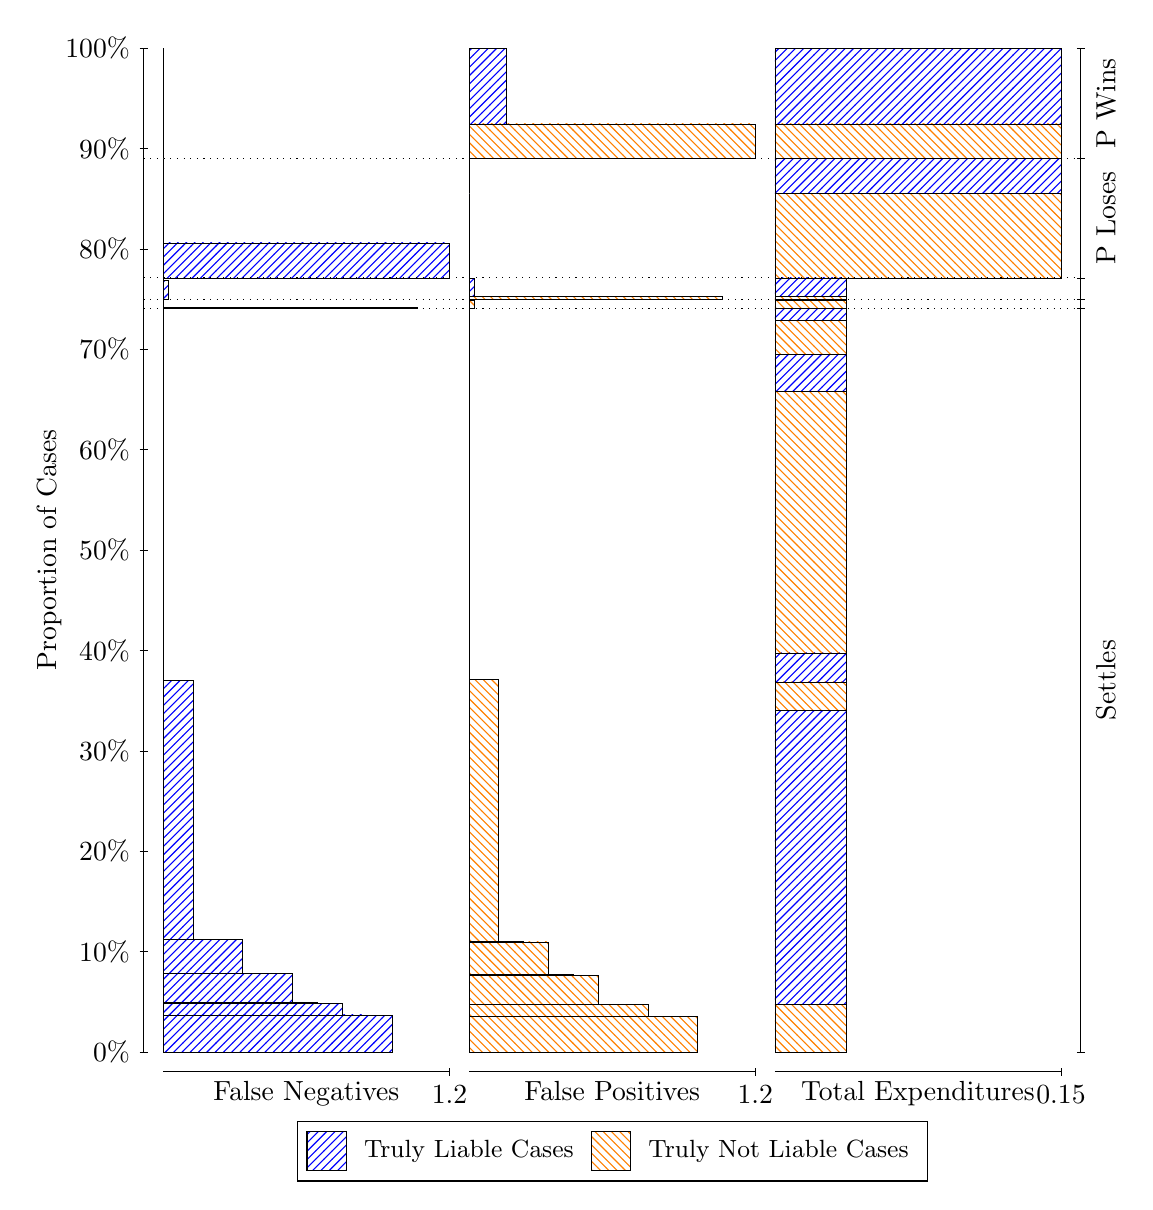
\begin{tikzpicture}
\draw[black, very thin] (1.5,1.75) -- (1.5,14.5);
\node[rotate=90, anchor=center] at (0.3, 8.125) {Proportion of Cases};
\draw[black, very thin] (1.45,1.75) -- (1.55,1.75);
\node[anchor=east] at (1.45, 1.75) {0\%};
\draw[black, very thin] (1.45,3.025) -- (1.55,3.025);
\node[anchor=east] at (1.45, 3.025) {10\%};
\draw[black, very thin] (1.45,4.3) -- (1.55,4.3);
\node[anchor=east] at (1.45, 4.3) {20\%};
\draw[black, very thin] (1.45,5.575) -- (1.55,5.575);
\node[anchor=east] at (1.45, 5.575) {30\%};
\draw[black, very thin] (1.45,6.85) -- (1.55,6.85);
\node[anchor=east] at (1.45, 6.85) {40\%};
\draw[black, very thin] (1.45,8.125) -- (1.55,8.125);
\node[anchor=east] at (1.45, 8.125) {50\%};
\draw[black, very thin] (1.45,9.4) -- (1.55,9.4);
\node[anchor=east] at (1.45, 9.4) {60\%};
\draw[black, very thin] (1.45,10.675) -- (1.55,10.675);
\node[anchor=east] at (1.45, 10.675) {70\%};
\draw[black, very thin] (1.45,11.95) -- (1.55,11.95);
\node[anchor=east] at (1.45, 11.95) {80\%};
\draw[black, very thin] (1.45,13.225) -- (1.55,13.225);
\node[anchor=east] at (1.45, 13.225) {90\%};
\draw[black, very thin] (1.45,14.5) -- (1.55,14.5);
\node[anchor=east] at (1.45, 14.5) {100\%};

\draw[black, very thin] (13.4,1.75) -- (13.4,14.5);
\draw[black, very thin] (13.35,1.75) -- (13.45,1.75);
\node[anchor=west] at (13.35, 1.75) {};
\draw[black, very thin] (13.35,11.197) -- (13.45,11.197);
\node[anchor=west] at (13.35, 11.197) {};
\draw[black, very thin] (13.35,11.31) -- (13.45,11.31);
\node[anchor=west] at (13.35, 11.31) {};
\draw[black, very thin] (13.35,11.582) -- (13.45,11.582);
\node[anchor=west] at (13.35, 11.582) {};
\draw[black, very thin] (13.35,13.094) -- (13.45,13.094);
\node[anchor=west] at (13.35, 13.094) {};
\draw[black, very thin] (13.35,14.5) -- (13.45,14.5);
\node[anchor=west] at (13.35, 14.5) {};

\draw[black, very thin, pattern color=blue, pattern=north east lines] (1.75,1.75) rectangle (4.6527,2.2168);
\draw[black, very thin, pattern color=blue, pattern=north east lines] (1.75,2.2168) rectangle (4.3368,2.22);
\draw[black, very thin, pattern color=blue, pattern=north east lines] (1.75,2.22) rectangle (4.0208,2.3712);
\draw[black, very thin, pattern color=blue, pattern=north east lines] (1.75,2.3712) rectangle (3.7049,2.3746);
\draw[black, very thin, pattern color=blue, pattern=north east lines] (1.75,2.3746) rectangle (3.7049,2.3757);
\draw[black, very thin, pattern color=blue, pattern=north east lines] (1.75,2.3757) rectangle (3.3889,2.7439);
\draw[black, very thin, pattern color=blue, pattern=north east lines] (1.75,2.7439) rectangle (3.073,2.7521);
\draw[black, very thin, pattern color=blue, pattern=north east lines] (1.75,2.7521) rectangle (2.7571,3.1814);
\draw[black, very thin, pattern color=blue, pattern=north east lines] (1.75,3.1814) rectangle (2.4411,3.1824);
\draw[black, very thin, pattern color=blue, pattern=north east lines] (1.75,3.1824) rectangle (2.1252,6.4683);
\draw[black, very thin, pattern color=orange, pattern=north west lines] (1.75,6.4683) rectangle (1.75,11.197);
\draw[black, very thin, pattern color=blue, pattern=north east lines] (1.75,11.197) rectangle (4.9687,11.207);
\draw[black, very thin, pattern color=orange, pattern=north west lines] (1.75,11.207) rectangle (1.75,11.31);
\draw[black, very thin, pattern color=blue, pattern=north east lines] (1.75,11.31) rectangle (1.8092,11.55);
\draw[black, very thin, pattern color=orange, pattern=north west lines] (1.75,11.55) rectangle (1.75,11.582);
\draw[black, very thin, pattern color=blue, pattern=north east lines] (1.75,11.582) rectangle (5.3833,12.025);
\draw[black, very thin, pattern color=orange, pattern=north west lines] (1.75,12.025) rectangle (1.75,13.094);
\draw[black, very thin, pattern color=orange, pattern=north west lines] (1.75,13.094) rectangle (1.75,13.537);
\draw[black, very thin, pattern color=blue, pattern=north east lines] (1.75,13.537) rectangle (1.75,14.5);
\draw[black, very thin, pattern color=orange, pattern=north west lines] (5.6333,1.75) rectangle (8.5361,2.2);
\draw[black, very thin, pattern color=orange, pattern=north west lines] (5.6333,2.2) rectangle (8.2201,2.2019);
\draw[black, very thin, pattern color=orange, pattern=north west lines] (5.6333,2.2019) rectangle (7.9042,2.3552);
\draw[black, very thin, pattern color=orange, pattern=north west lines] (5.6333,2.3552) rectangle (7.5882,2.3593);
\draw[black, very thin, pattern color=orange, pattern=north west lines] (5.6333,2.3593) rectangle (7.2723,2.7244);
\draw[black, very thin, pattern color=orange, pattern=north west lines] (5.6333,2.7244) rectangle (6.9563,2.7295);
\draw[black, very thin, pattern color=orange, pattern=north west lines] (5.6333,2.7295) rectangle (6.9563,2.7324);
\draw[black, very thin, pattern color=orange, pattern=north west lines] (5.6333,2.7324) rectangle (6.6404,3.1489);
\draw[black, very thin, pattern color=orange, pattern=north west lines] (5.6333,3.1489) rectangle (6.3245,3.1518);
\draw[black, very thin, pattern color=orange, pattern=north west lines] (5.6333,3.1518) rectangle (6.0085,6.4785);
\draw[black, very thin, pattern color=blue, pattern=north east lines] (5.6333,6.4785) rectangle (5.6333,11.197);
\draw[black, very thin, pattern color=orange, pattern=north west lines] (5.6333,11.197) rectangle (5.6926,11.3);
\draw[black, very thin, pattern color=blue, pattern=north east lines] (5.6333,11.3) rectangle (5.6333,11.31);
\draw[black, very thin, pattern color=orange, pattern=north west lines] (5.6333,11.31) rectangle (8.852,11.342);
\draw[black, very thin, pattern color=blue, pattern=north east lines] (5.6333,11.342) rectangle (5.6926,11.582);
\draw[black, very thin, pattern color=orange, pattern=north west lines] (5.6333,11.582) rectangle (5.6333,12.65);
\draw[black, very thin, pattern color=blue, pattern=north east lines] (5.6333,12.65) rectangle (5.6333,13.094);
\draw[black, very thin, pattern color=orange, pattern=north west lines] (5.6333,13.094) rectangle (9.2667,13.537);
\draw[black, very thin, pattern color=blue, pattern=north east lines] (5.6333,13.537) rectangle (6.1072,14.5);
\draw[black, very thin, pattern color=orange, pattern=north west lines] (9.5167,1.75) rectangle (10.425,2.3593);
\draw[black, very thin, pattern color=blue, pattern=north east lines] (9.5167,2.3593) rectangle (10.425,6.0837);
\draw[black, very thin, pattern color=orange, pattern=north west lines] (9.5167,6.0837) rectangle (10.425,6.4488);
\draw[black, very thin, pattern color=blue, pattern=north east lines] (9.5167,6.4488) rectangle (10.425,6.817);
\draw[black, very thin, pattern color=orange, pattern=north west lines] (9.5167,6.817) rectangle (10.425,10.144);
\draw[black, very thin, pattern color=blue, pattern=north east lines] (9.5167,10.144) rectangle (10.425,10.611);
\draw[black, very thin, pattern color=orange, pattern=north west lines] (9.5167,10.611) rectangle (10.425,11.038);
\draw[black, very thin, pattern color=blue, pattern=north east lines] (9.5167,11.038) rectangle (10.425,11.197);
\draw[black, very thin, pattern color=orange, pattern=north west lines] (9.5167,11.197) rectangle (10.425,11.3);
\draw[black, very thin, pattern color=blue, pattern=north east lines] (9.5167,11.3) rectangle (10.425,11.31);
\draw[black, very thin, pattern color=orange, pattern=north west lines] (9.5167,11.31) rectangle (10.425,11.342);
\draw[black, very thin, pattern color=blue, pattern=north east lines] (9.5167,11.342) rectangle (10.425,11.582);
\draw[black, very thin, pattern color=orange, pattern=north west lines] (9.5167,11.582) rectangle (13.15,12.65);
\draw[black, very thin, pattern color=blue, pattern=north east lines] (9.5167,12.65) rectangle (13.15,13.094);
\draw[black, very thin, pattern color=orange, pattern=north west lines] (9.5167,13.094) rectangle (13.15,13.537);
\draw[black, very thin, pattern color=blue, pattern=north east lines] (9.5167,13.537) rectangle (13.15,14.5);
\draw[black, dotted] (1.5,11.197) -- (13.4,11.197);
\draw[black, dotted] (1.5,11.31) -- (13.4,11.31);
\draw[black, dotted] (1.5,11.582) -- (13.4,11.582);
\draw[black, dotted] (1.5,13.094) -- (13.4,13.094);
\draw[black, very thin] (1.75,1.5) -- (5.3833,1.5);
\node[anchor=north] at (3.5667, 1.5) {False Negatives};
\draw[black, very thin] (5.3833,1.45) -- (5.3833,1.55);
\node[anchor=north] at (5.3833, 1.45) {1.2};

\draw[black, very thin] (5.6333,1.5) -- (9.2667,1.5);
\node[anchor=north] at (7.45, 1.5) {False Positives};
\draw[black, very thin] (9.2667,1.45) -- (9.2667,1.55);
\node[anchor=north] at (9.2667, 1.45) {1.2};

\draw[black, very thin] (9.5167,1.5) -- (13.15,1.5);
\node[anchor=north] at (11.333, 1.5) {Total Expenditures};
\draw[black, very thin] (13.15,1.45) -- (13.15,1.55);
\node[anchor=north] at (13.15, 1.45) {0.15};

\node[black, centered, rotate=90] at (13.72, 6.4734) {Settles};


\node[black, centered, rotate=90] at (13.72, 12.338) {P Loses};
\node[black, centered, rotate=90] at (13.72, 13.797) {P Wins};

\draw (7.449999999999999,1.5) node[draw=none] (baseCoordinate) {};
\begin{scope}[align=center]
        \matrix[scale=0.5, draw=black, below=0.5cm of baseCoordinate, nodes={draw}, column sep=0.1cm]{
            \node[rectangle, draw, minimum width=0.5cm, minimum height=0.5cm, pattern=north east lines, pattern color=blue] {}; &
            \node[draw=none, font=\small] (B) {Truly Liable Cases}; &
            \node[rectangle, draw, minimum width=0.5cm, minimum height=0.5cm, pattern=north west lines, pattern color=orange] {}; &
            \node[draw=none, font=\small] (B) {Truly Not Liable Cases}; \\
            };
\end{scope}

\end{tikzpicture}
\end{document}